\documentclass[10pt]{beamer}
\usetheme{Warsaw}
\usepackage[T1]{fontenc}
\usepackage[utf8]{inputenc}
\usepackage{chronosys}
\usepackage{hyperref}

\title{Waterfall}
\author{Team Niagara\_falls}
\date{}

\begin{document}
\frame{\titlepage}
\begin{frame}
    \tableofcontents
\end{frame}

% Partie 1:


\section{Introduction and History}
\subsection{Introduction}
\begin{frame}
\frametitle{Introduction and History}
\framesubtitle{Introduction}
\begin{itemize}
    \item Linear sequential phases
    \item Used in engineering design
    \item In software development: 
    \begin{itemize}
        \item earliest SDLC approach
        \item the less iterative and flexible approaches
    \end{itemize}    
\end{itemize}
\end{frame}

\subsection{History}
\begin{frame}
\frametitle{Introduction and History}
\framesubtitle{History}
\startchronology
[startyear=1950,stopyear=1990]
\chronoevent[textwidth=3cm]{1956}{\footnotesize First presentation}
\chronoevent[textwidth=3cm]{1970}{\footnotesize First citation in an article}
\chronoevent[textwidth=3cm]{1985}{\footnotesize United States Department of Defense captured this approach}
\stopchronology
    
\end{frame}


% Partie 2:
\section{Presentation of the method}
\begin{frame}
\setbeamertemplate{blocks}[rounded][shadow=false]
\frametitle{Waterfall method}
\begin{figure}
    \centering
    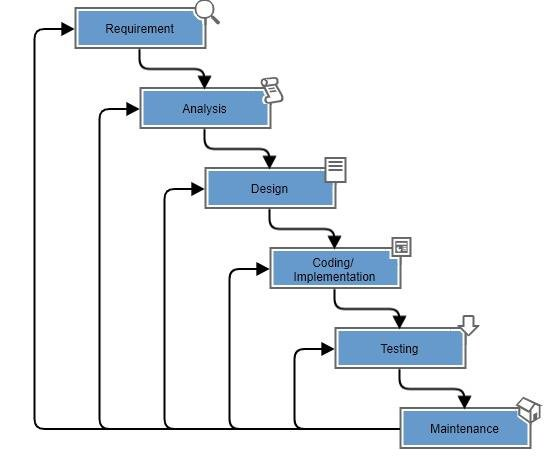
\includegraphics[width=0.8\linewidth]{waterfall method.png}
    \caption{waterfall model}
\end{figure}
\end{frame}
\begin{frame}
\setbeamertemplate{blocks}[rounded][shadow=false]
\frametitle{Requirement}

\begin{block}{system requirement}
\begin{itemize}

    \item Deadline
        
    \item Budget
           
\end{itemize}
\end{block}

\begin{block}{software requirement}
\begin{itemize}

    \item Functionality
        
    \item User interface
        
    \item Support
        
\end{itemize}
  
\end{block}
\end{frame}
\begin{frame}
\setbeamertemplate{blocks}[rounded][shadow=false]
\frametitle{Analysis and Design}

\begin{block}{Analysis}
\begin{itemize}

    \item Structure
        
    \item Create a model
        
    \item Technical resources
        
\end{itemize}
\end{block}
\begin{block}{Design}
\begin{itemize}

    \item language
        
    \item Class
        
    \item Libraries
    
    \item Main function
        
\end{itemize}
\end{block}
\end{frame}


% Partie 3:
\begin{frame}
\setbeamertemplate{blocks}[rounded][shadow=false]
\frametitle{Coding}
\begin{block}{Coding}
At this stage we start implementing the project,using the model and logic found during the last phase.The project will most likely be coded in smaller components before being put together.
\end{block}

\begin{block}{Testing}
After coding we need to test our product to see if it works well,do some quality insurance and debug.
\end{block}
\end{frame}

\begin{frame}
\setbeamertemplate{blocks}[rounded][shadow=false]
\frametitle{Last operation}
\begin{block}{Deployment}
The product is judged finished and deployed into action.
\end{block}
\begin{block}{Maintenance}
Correction of bug and performance maintenance to improve or fix the final product. That can lead to a series of patches. 
\end{block}
    

\end{frame}


% Partie 4:

\section{Advantages and Criticisms}
\subsection{Pros:}

\begin{frame}
\setbeamertemplate{blocks}[rounded][shadow=false]
\frametitle{Advantages}

\begin{block}{Simple and easy to understand}
Its linear and sequential nature makes it easy to comprehend, especially for stakeholders who are not familiar with software development processes.
\end{block}

\begin{block}{Clear milestones and deliverables}
Each phase has well-defined deliverables and milestones, making it easier to track progress and manage expectations.
\end{block}

\begin{block}{Early detection of issues}
Because requirements are established upfront, any potential issues can be identified early in the process, reducing the likelihood of major changes later on.
\end{block}

\begin{block}{Structured approach}
The rigid structure ensures that each phase is completed before moving on to the next, which can provide a sense of security and stability.
\end{block}

\end{frame}

\subsection{Cons:}

\begin{frame}
\setbeamertemplate{blocks}[rounded][shadow=false]
\frametitle{Criticisms}

\begin{block}{Limited flexibility}
The linear nature of the Waterfall model makes it difficult to accommodate changes once a phase is completed.
\end{block}

\begin{block}{Late testing}
Testing occurs towards the end of the development process, which means that defects may not be discovered until late stages, leading to higher costs and risks.
\end{block}

\begin{block}{Client involvement limited to early stages}
This involvement typically occurs primarily in the requirements phase, which can lead to misunderstandings or mismatches between client expectations and the final product.
\end{block}

\end{frame}

% Partie 5:
\section{Examples of Waterfall Projects}
\begin{frame}
\frametitle{Examples of Waterfall Projects}
\begin{block}{Construction Projects}
These projects typically involve linear and sequential phases such as planning, design, pre-construction, construction, and closeout.
\end{block}

\begin{block}{Healthcare Projects}
These projects involve phases like planning, requirements gathering, design, implementation, testing, deployment, and maintenance of medical grade projects, systems and solutions.
\end{block}

\begin{block}{Manufacturing Projects}
Manufacturing projects involve the production of physical goods. Phases include planning, design, procurement, production, and delivery.
\end{block}
\end{frame}

% Partie 6:
\section{Example of the Failure of a Waterfall Project}
\begin{frame}
\frametitle{Example of a Failure of a Waterfall Project}
In 2012, the California Judicial Council has suspended the California Court Case Management System (CCMS), a software project aimed at modernizing the state's trial courts due to budget constraints despite already spending hundreds of millions of dollars on the project. The CCMS project had faced criticism and skepticism for years, with concerns raised about its potential obsolescence and failure to realize expected returns on investment.
\end{frame}


\section{References}
\begin{frame}
    \setbeamertemplate{blocks}[rounded][shadow=false]
    \frametitle{References}
    \begin{itemize}

        \item \href{https://en.wikipedia.org/wiki/Waterfall_model}{wikipedia/waterfall\_model}
            
        \item \href{https://www.techtarget.com/searchsoftwarequality/definition/waterfall-model}{techtarget/waterfall\_model}
            
        \item \href{https://en.ryte.com/wiki/Waterfall_Model}{ryte/waterfall\_model}
        
        \item \href{https://www.tutorialspoint.com/sdlc/sdlc_waterfall_model.htm}{tutorialspoint/waterfall\_model}
            
    \end{itemize}

\end{frame}

\end{document}
